\newpage
\everymath{\color{toancuabi}}
\graphicspath{{../timhieucungbi/quansatcackhoihinh/}}
\begingroup
\AddToShipoutPicture*{\put(90,548){
\includegraphics[scale=0.75]{tieude3}}} 
\centering
\endgroup

	$1.$ Khối hình dưới đây được quan sát từ ba hướng khác nhau.
	\begin{center}
		\begin{thBox}
			\begin{multicols}{2}
				\begin{figure}[H]
					\centering
					\vspace*{-10pt}
					\captionsetup{labelformat= empty, justification=centering}
					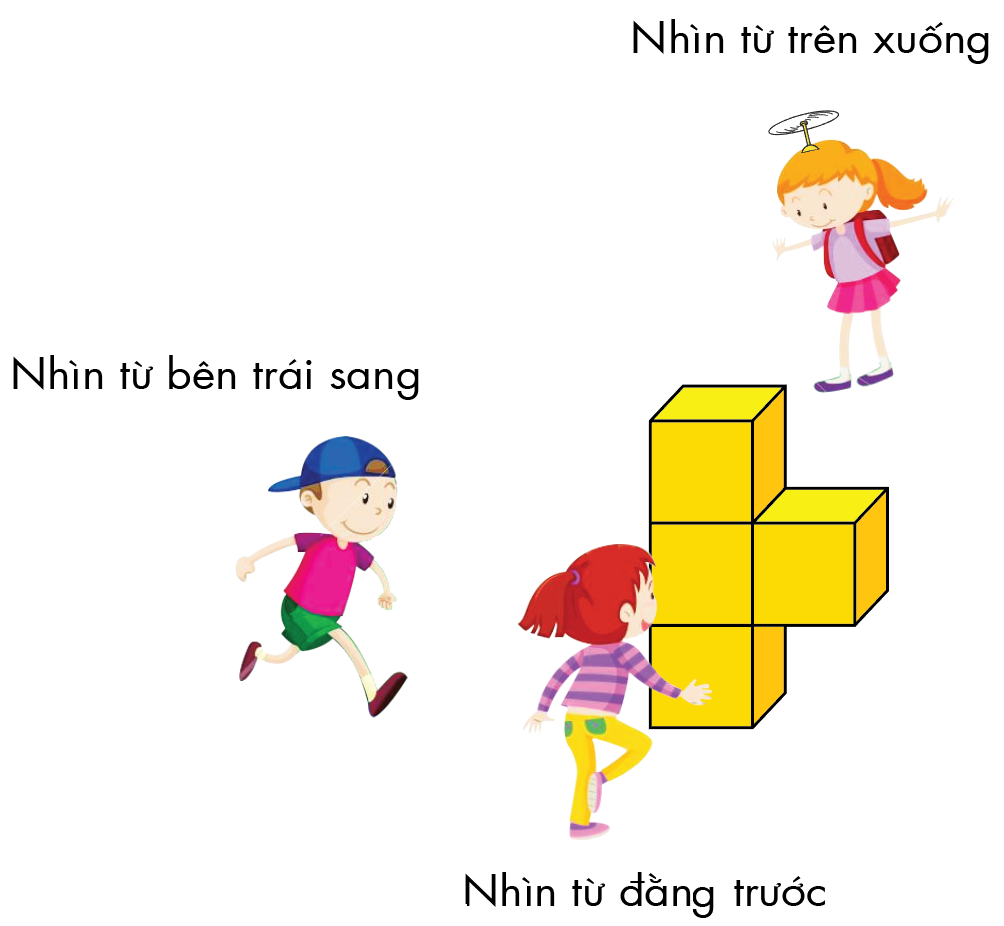
\includegraphics[width=0.475\textwidth]{1}
					\vspace*{-10pt}
				\end{figure}
				\vspace*{-16pt}
				Khi nhìn từ đằng trước, sẽ nhìn thấy hình sau:
				\begin{figure}[H]
					\centering
					\captionsetup{labelformat= empty, justification=centering}
					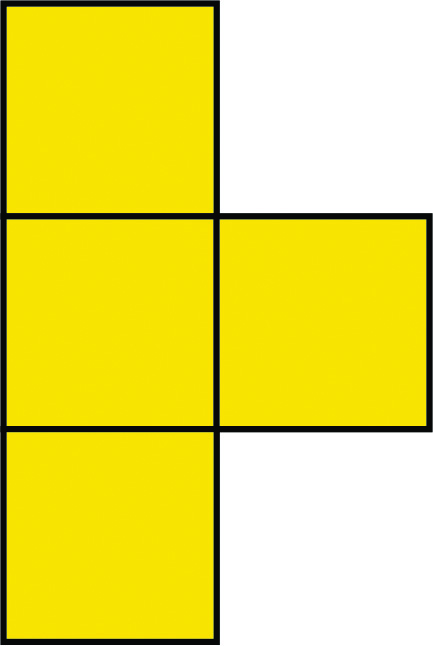
\includegraphics[width=0.15\textwidth]{2}
					\vspace*{5pt}
				\end{figure}
			\end{multicols}
		\end{thBox}
	\end{center}
	Nối hình quan sát được với hướng nhìn tương ứng.
	\begin{center}
		\setlength{\tabcolsep}{18pt}
		\arrayrulecolor{ocre}
		\renewcommand{\arraystretch}{2}
		\begin{tabularx}{1\textwidth} { 
				 >{\centering\arraybackslash}X 
				 >{\centering\arraybackslash}X}
%			\hline
			Các hướng quan sát&	Hình nhìn thấy\\
			\hline
			Nhìn từ trên xuống&\adjustimage{angle = 90, scale = 0.5,valign = M}{4}\\
%			\hline	 
			Nhìn từ bên trái sang&\adjustimage{scale= 0.12, valign = M}{5}\\
%			\hline
		\end{tabularx}
	\end{center}
	$2.$ Cho khối hình dưới đây.
	\begin{multicols}{2}
		\begin{thBox}
			\begin{figure}[H]
				\centering
				\vspace*{-10pt}
				\captionsetup{labelformat= empty, justification=centering}
				
\includegraphics[scale=0.25]{6}
				\vspace*{5pt}
			\end{figure}
		\end{thBox}
	\begin{figure}[H]
		\centering
%		\vspace*{-10pt}
		\captionsetup{labelformat= empty, justification=centering}
		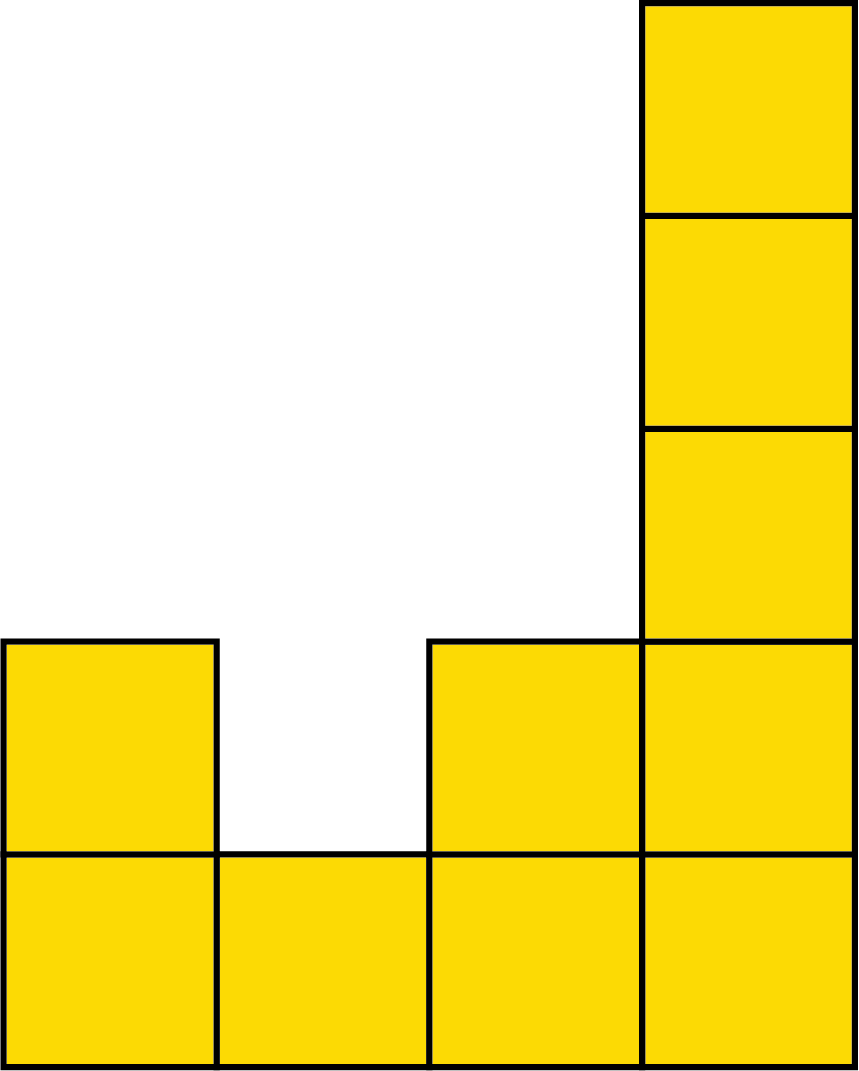
\includegraphics[width=0.18\textwidth]{7a}\,
		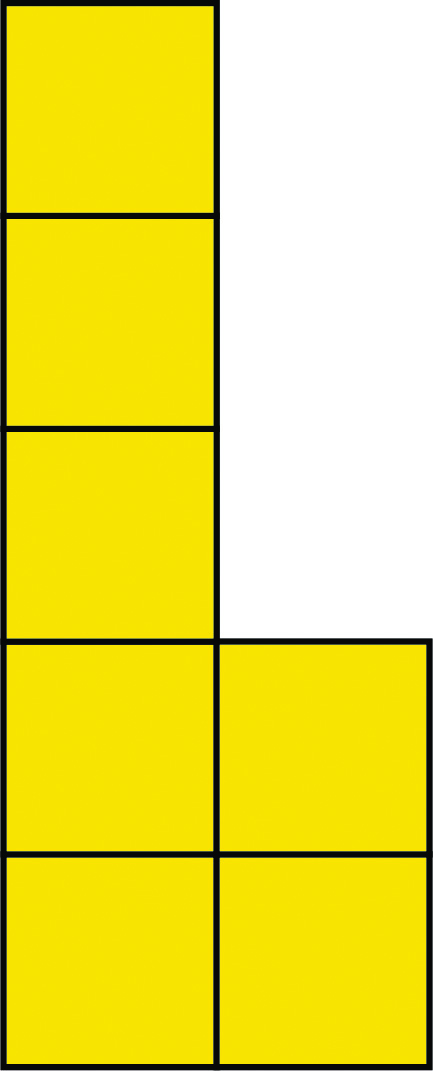
\includegraphics[width=0.08\textwidth]{7b}\,
		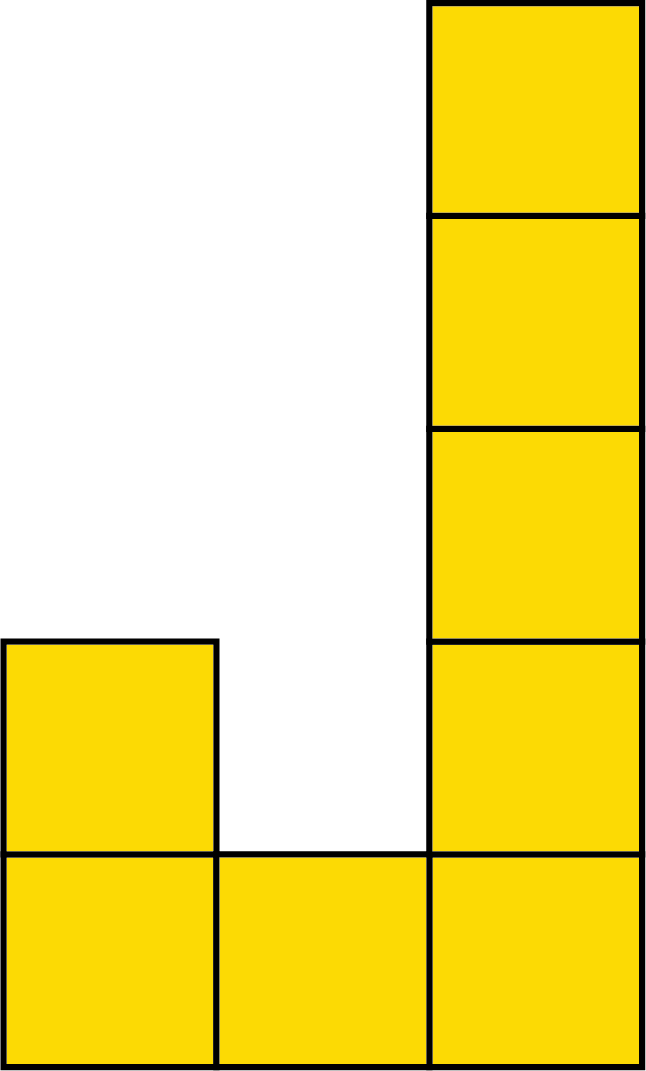
\includegraphics[width=0.13\textwidth]{7c}
		\caption{{\color[named]{toancuabi}\hspace*{5pt}(A)\hspace*{50pt} (B) \hspace*{35pt}(C)}}
		\vspace*{-5pt}
	\end{figure} 
	\end{multicols}
	Khi nhìn khối hình trên từ {\color[named]{toancuabi}bên trái} sang, em nhìn thấy hình nào?
	\vskip 0.1cm
	$3.$ Hình trong khung là hình nhìn từ {\color[named]{toancuabi}bên phải} sang của khối hình nào trong các khối hình sau?
	\vskip 0.1cm
%	\vspace*{5pt}
	\begin{adjustwidth}{0pt}{200pt}
		\begin{thBox}
			\begin{figure}[H]
				\centering
				\vspace*{5pt}
				\captionsetup{labelformat= empty, justification=centering}
				
\includegraphics[scale=0.3]{8}
				\vspace*{20pt}
			\end{figure}
		\end{thBox}
	\end{adjustwidth}
	
	\insertpic{170}{425}{0.3}{9a}
	\insertpic{220}{425}{0.3}{9b}
	\insertpic{315}{425}{0.3}{9c}
	\vspace*{-25pt}
	{\color[named]{toancuabi}\hspace*{115pt} (A) \hspace*{45pt} (B) \hspace*{45pt} (C)}
	\vskip 0.1cm
	\vspace*{10pt}
	$4.$ Bạn Lenny quan sát một khối hình từ $3$ hướng khác nhau thì thu được các hình như sau. 
	\begin{center}
%		\setlength{\tabcolsep}{18pt}
		\arrayrulecolor{ocre}
		\renewcommand{\arraystretch}{2}
		\begin{tabularx}{1\textwidth} { 
				>{\centering\arraybackslash}X 
				>{\centering\arraybackslash}X
				>{\centering\arraybackslash}X}
%			\hline
			Nhìn từ trên xuống&	Nhìn từ bên phải sang& Nhìn từ bên trái sang\\
%			\hline
			\adjustimage{scale = 0.5,valign=M}{10a}&\adjustimage{scale = 0.5,valign=M}{10b}&\adjustimage{scale = 0.5,valign=M}{10c}\\
%			\hline
		\end{tabularx}
	\end{center}
	Hỏi khối hình nào có thể là khối hình của Lenny? 
		\begin{center}
		\arrayrulecolor{ocre}
		\renewcommand{\arraystretch}{2}
		\begin{tabularx}{1\textwidth} { 
				 >{\centering\arraybackslash}X 
				 >{\centering\arraybackslash}X
				 >{\centering\arraybackslash}X}
			(A)\quad\adjustimage{width=0.2\textwidth,valign=M}{11a}&(B)\quad\adjustimage{width=0.2\textwidth,valign=M}{11b}&(C)\quad\adjustimage{width=0.2\textwidth,valign=M}{11c}\\
		\end{tabularx}
	\end{center}  
	$5.$ Em hãy vẽ hình thu được khi nhìn khối hình dưới đây từ $3$ hướng khác nhau.
	
	\begin{adjustwidth}{100pt}{0pt}
		\vspace*{-5pt}
			\arrayrulecolor{ocre}
			\renewcommand{\arraystretch}{2}
			\begin{tabularx}{0.7\textwidth} { 
					|>{\centering\arraybackslash}X 
					>{\centering\arraybackslash}X
					>{\centering\arraybackslash}X|}
				\hline
				Nhìn từ đằng trước&	Nhìn từ trên xuống& Nhìn từ bên trái sang\\
				\hline
				&&\\
				\hline
			\end{tabularx}
	\end{adjustwidth}
	\vspace*{10pt}
	\insertpic{65}{75}{0.3}{12}
	$6.$ Ann quan sát tủ quần áo của mình từ $3$ hướng khác nhau.
	  \begin{figure}[H]
	  	\centering
	  	\vspace*{-5pt}
	  	\captionsetup{labelformat= empty, justification=centering}
	  	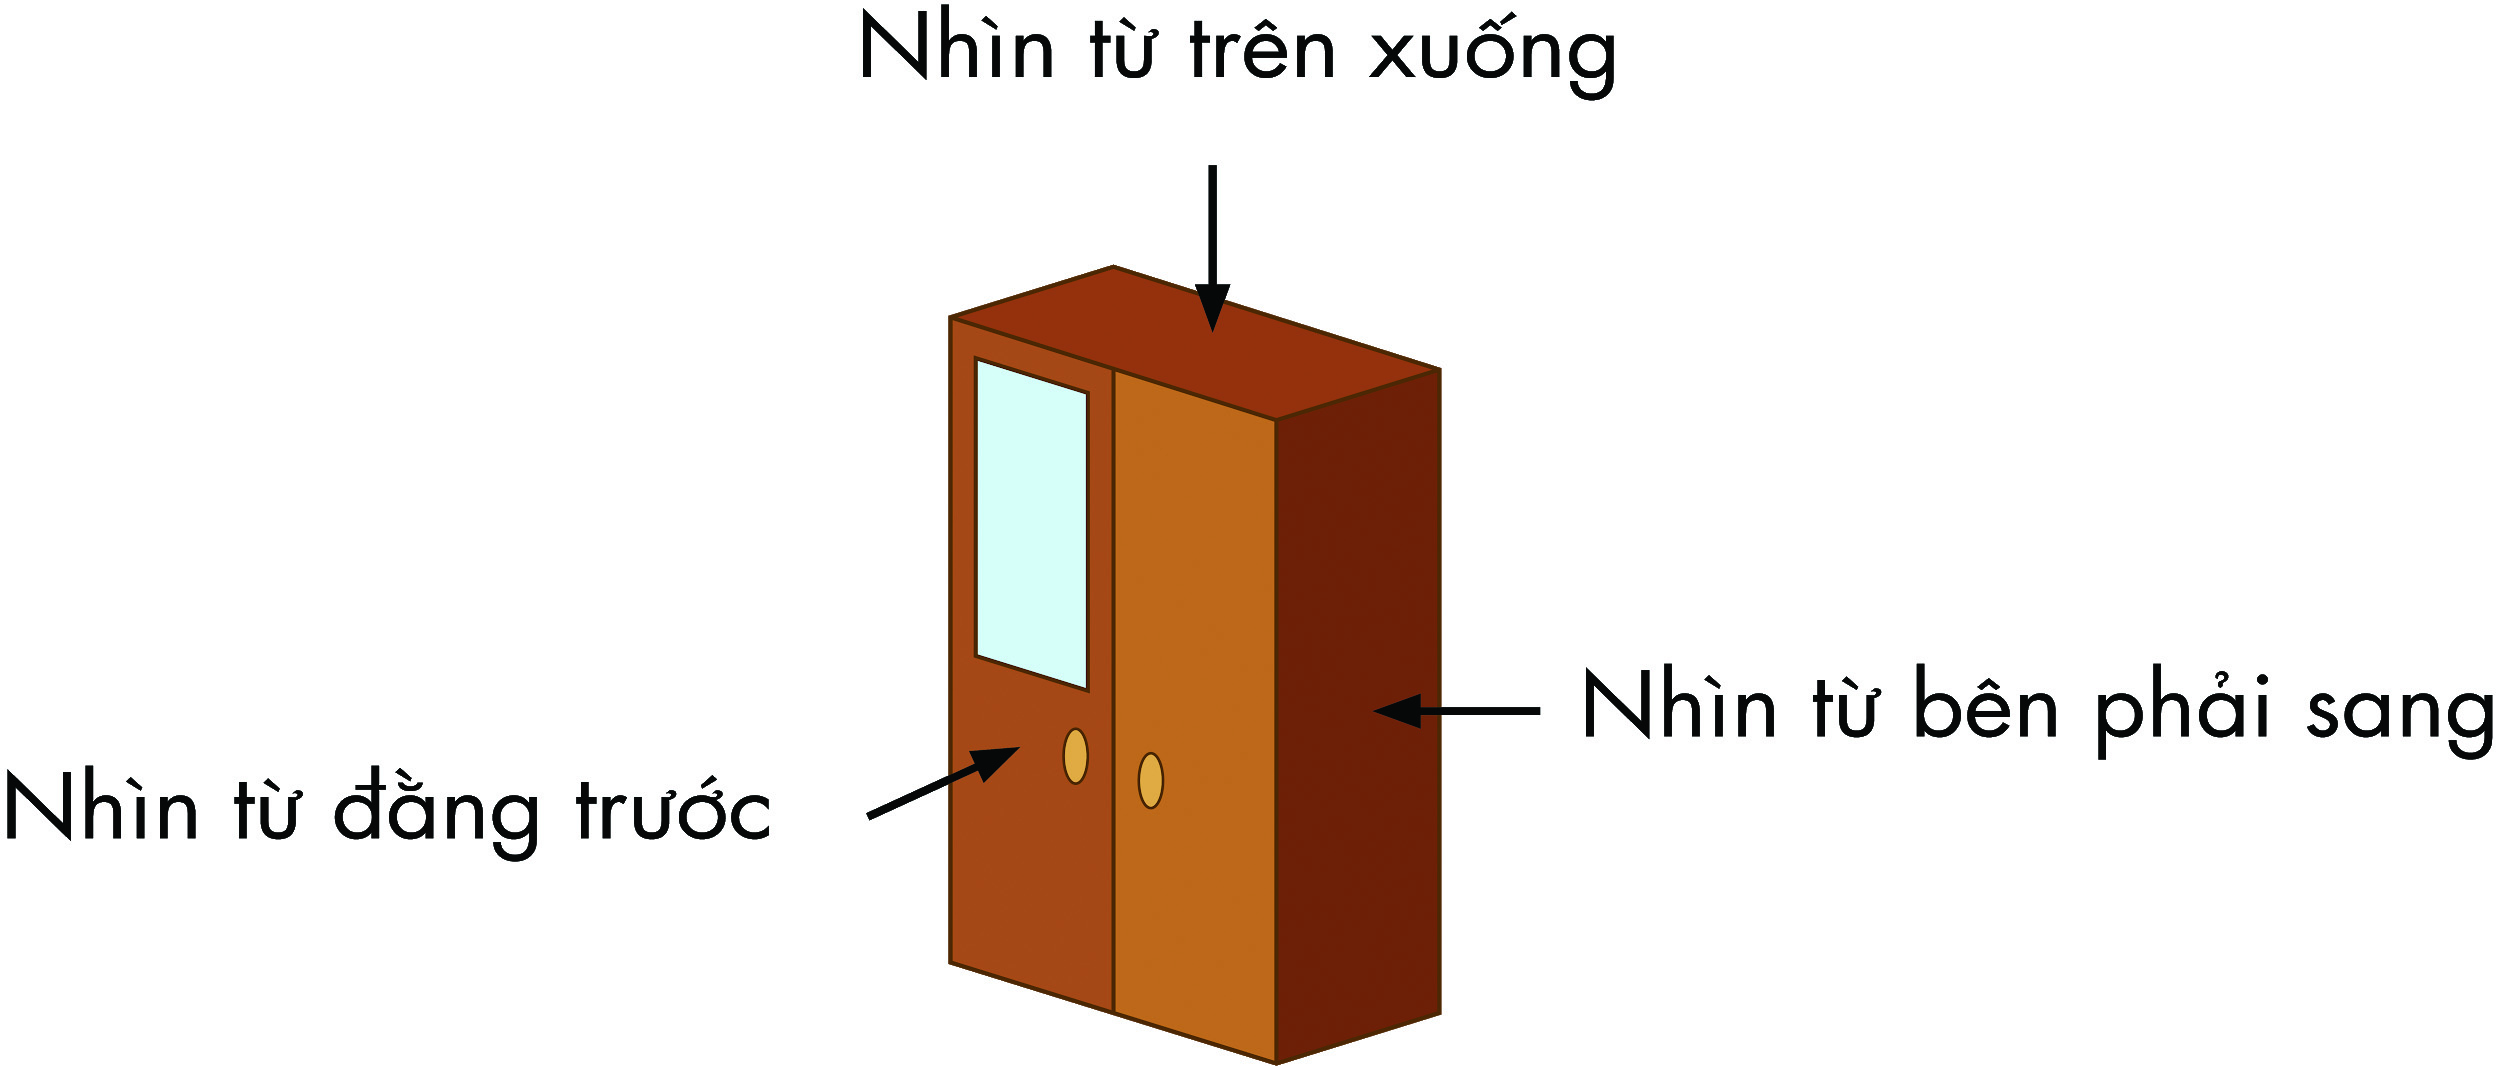
\includegraphics[width=0.75\textwidth]{14}
	  	\vspace*{-15pt}
	  \end{figure}
	Nối hình Ann quan sát được với hướng nhìn tương ứng.
	\begin{center}
		\setlength{\tabcolsep}{18pt}
		\arrayrulecolor{ocre}
		\renewcommand{\arraystretch}{2}
		\begin{tabularx}{1\textwidth} { 
				>{\centering\arraybackslash}X 
				>{\centering\arraybackslash}X}
%			\hline
			Các hướng quan sát&	Hình Ann nhìn thấy\\
			\hline
			Nhìn từ trên xuống&\adjustimage{scale = 1,valign=M}{15a}\\
			%			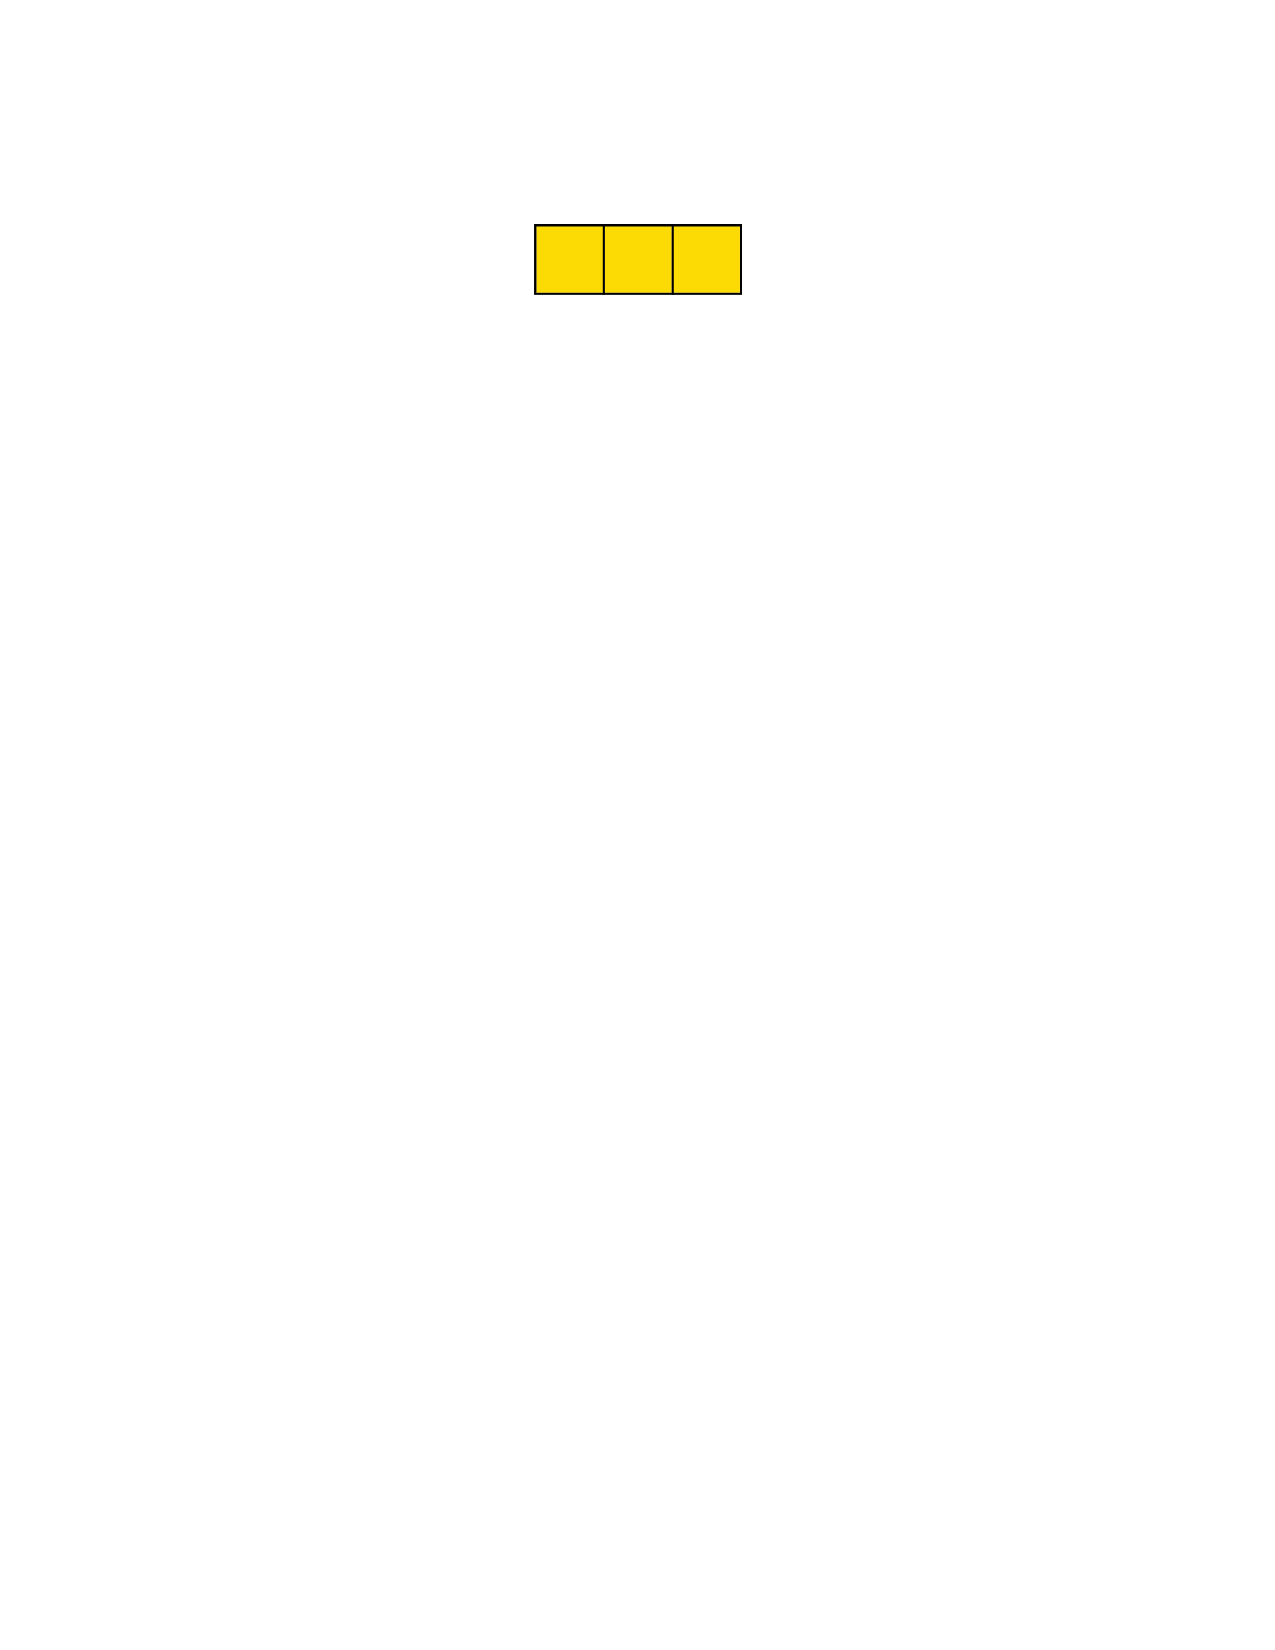
\includegraphics[scale= 0.2]{4}\\ 
%			\hline	 
			Nhìn từ bên phải sang&\adjustimage{scale= 1, valign = M}{15b}\\
%			\hline
			Nhìn từ đằng trước&\adjustimage{scale= 1, valign = M}{15c}\\
%			\hline
		\end{tabularx}
	\end{center}
	$7.$ Khi nhìn cùng một khối hình từ các hướng khác nhau, ta nhìn thấy các hình như dưới đây:
	\begin{center}
%		\setlength{\tabcolsep}{18pt}
		\arrayrulecolor{ocre}
		\renewcommand{\arraystretch}{2}
		\begin{tabularx}{1\textwidth} { 
				>{\centering\arraybackslash}X 
				>{\centering\arraybackslash}X
				>{\centering\arraybackslash}X
				>{\centering\arraybackslash}X
				>{\centering\arraybackslash}X}
%			\hline
			Nhìn từ đằng trước&	Nhìn từ trên xuống &Nhìn từ bên phải sang&Nhìn từ bên trái sang& Nhìn từ đằng sau\\
%			\hline
			\adjustimage{scale = 0.35,valign=M}{16a}&\adjustimage{scale = 0.35,valign=M}{16b}&
			\adjustimage{scale= 0.35, valign = M}{16c}&\adjustimage{scale= 0.35, valign = M}{16d}&\adjustimage{scale= 0.35, valign = M}{16a}\\
%			\hline
		\end{tabularx}
	\end{center}
	\vspace*{10pt}
	$a)$ Hỏi khối hình đó có thể là khối hình nào sau đây? 
	  	\begin{center}
	  	\arrayrulecolor{ocre}
	  	\renewcommand{\arraystretch}{2}
	  	\begin{tabularx}{1\textwidth} { 
	  			>{\centering\arraybackslash}X 
	  			>{\centering\arraybackslash}X
	  			>{\centering\arraybackslash}X}
	  		%			\hline
	  		\adjustimage{width=0.2\textwidth,valign=M}{19a}&\adjustimage{width=0.2\textwidth,valign=M}{19b}&\adjustimage{width=0.25\textwidth,valign=M}{19c}\\
	  		%			\hline
	  		(A)&(B)&(C)
	  	\end{tabularx}
	  \end{center} 
	$b)$ Có bao nhiêu khối hình khác nhau như vậy? Chú ý, với nhìn từ trên xuống, ta xét là đứng từ phía sau hướng về phía trước và nhìn từ trên xuống.
	\begin{figure}[H]
		\centering
		\vspace*{-5pt}
		\captionsetup{labelformat= empty, justification=centering}
		
\includegraphics[width=0.4\textwidth]{20}
		\vspace*{-10pt}
	\end{figure}